\section{feedforward フィルタの実装}
    \subsection{複素係数 feedforward フィルタの乗算回路の削減}
        \subsubsection{対象とするフィルタの定義式}
            \newcommand*{\xIn}{x_\text{i}}
            \newcommand*{\xOut}{x_\text{o}}
            入出力が次の関係式で与えられる feedforward フィルタを ASIC, FPGA に実装することを考える。
            \[ \xOut(n) = \sum_{m=0}^{\Ntp-1} h(m)\xIn(n-m) \tag{1} \]
            ここに $\xIn,\xOut:\integers\to\complexNumbers$ はそれぞれ入力と出力の信号であり,$h:\integers\to\complexNumbers$ はフィルタのインパルス応答である。$\Ntp$ はタップ数である。
            定義通りに愚直に計算すると次のいずれかとなる(有限桁実数乗算回路の総数は等しい):
            \begin{enumerate}[label=(\alph*)]
                \item 1 タップあたり有限桁実数乗算回路(以下では混乱の惧れが無い限り,単に「乗算回路」と呼ぶ)を 4 個用いる $\Ntp$ タップの複素係数フィルタ 1 個
                \item 1 タップあたり乗算回路を 1 個用いる $\Ntp$ タップの有限桁実数係数フィルタ 4 個
            \end{enumerate}
            (a) の構成に対しては,よく知られているように複素数同士の積を(加算回路の増加と引き換えに)実数乗算回路 3 個で実現できる。
            本節では (b) の構成に対して,タップ数を変えずに(加算回路の増加と引き換えに)有限桁実数係数フィルタの個数を 3 に削減する方法を示す。
        \subsubsection{導出}
            \label{複素係数 feedforward フィルタの乗算回路の削減_導出}
            \newcommand*{\xInReal}{x_\text{i,r}}
            \newcommand*{\xInImag}{x_\text{i,i}}
            \newcommand*{\xOutReal}{x_\text{o,r}}
            \newcommand*{\xOutImag}{x_\text{o,i}}
            \newcommand*{\hReal}{h_\text{r}}
            \newcommand*{\hImag}{h_\text{i}}
            $\xIn$ の実部と虚部をそれぞれ $\xInReal$ と $\xInImag$,$\xOut$ の実部と虚部をそれぞれ $\xOutReal$ と $\xOutImag$,$h$ の実部と虚部をそれぞれ $\hReal$ と $\hImag$ とする。
            式 (1) より次式を得る。
            \[
                \begin{cases}
                    \xOutReal(n) = \sum_{m=0}^{\Ntp-1} \hReal(m)\xInReal(n-m) - \sum_{m=0}^{\Ntp-1} \hImag(m)\xInImag(n-m) = \hReal * \xInReal - \hImag * \xInImag \\
                    \xOutImag(n) = \sum_{m=0}^{\Ntp-1} \hReal(m)\xInImag(n-m) + \sum_{m=0}^{\Ntp-1} \hImag(m)\xInReal(n-m) = \hImag * \xInReal + \hReal * \xInImag
                \end{cases}
            \]
            \newcommand*{\hSum}{h_\text{s}}
            \newcommand*{\hDiff}{h_\text{d}}
            \newcommand*{\xSum}{x_\text{s}}
            \newcommand*{\xAlpha}{x_\text{\alpha}}
            \newcommand*{\xBeta}{x_\text{\beta}}
            \newcommand*{\xGamma}{x_\text{\gamma}}
            ここで $\hSum,\;\hDiff,\;\xSum,\;\xAlpha,\;\xBeta,\;\xGamma$ を次の通り定義する。
            \[ \hSum \coloneq \hReal + \hImag,\quad \hDiff \coloneq \hReal - \hImag,\quad \xSum \coloneq \xInReal + \xInImag,\quad \xAlpha \coloneq \hSum * \xInReal,\quad \xBeta \coloneq \hDiff * \xInImag, \quad \xGamma \coloneq \hImag * \xSum \]
            上記の下で次式が成り立つ(畳み込みの交換法則に留意すべし)。
            \begin{align*}
                \xAlpha - \xGamma &= (\hReal + \hImag) * \xInReal - \hImag * (\xInReal + \xInImag) = \xOutReal \\
                \xBeta + \xGamma &= (\hReal - \hImag) * \xInImag + \hImag * (\xInReal + \xInImag) = \xOutImag
            \end{align*}
            次のブロック図は上式の計算過程を示している。
            \begin{figure}[H]
                \centering
                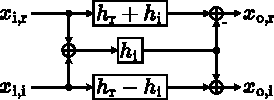
\includegraphics[keepaspectratio, scale=1]
                {\currfiledir/figs/mult_reduction_for_cplx_fd_fwd_flt.pdf}
                \caption{3 個の feedforward フィルタで実現された系}
            \end{figure}